To visualize and compare the behaviour of the flux of the \search\ and \temp\ images, the value distribution for the four transients presented in \autoref{fig:examples_no_normalization} is shown as a violin plot in \autoref{fig:violinplot}. The first transient on the left is labeled as ``bogus'', the \search\ distribution pixel values are in general greater, positive and non-zero center than the values for \temp, the same behaviour is observed to the last transient on the right, but this one is labeled as ``real''. This same comparison can be applied to the transients plotted on the middle of \autoref{fig:violinplot}, both show similar distributions, however one is ``bogus'' and the other is ``real''. For the four transients presented the pixel values have long tails, outside the $\mu \pm 3\sigma$ values. The scaling of the \search\ and \temp\ images for the four transients, according to the description given in \autoref{subsec:scaling} is visualized in \autoref{fig:violinplotscaling}. 

%Due to the long tails presented in each image, the similarities observed in \autoref{fig:violinplot} are not longer visible after the scaling.
\begin{figure*}[h]
    \centering
    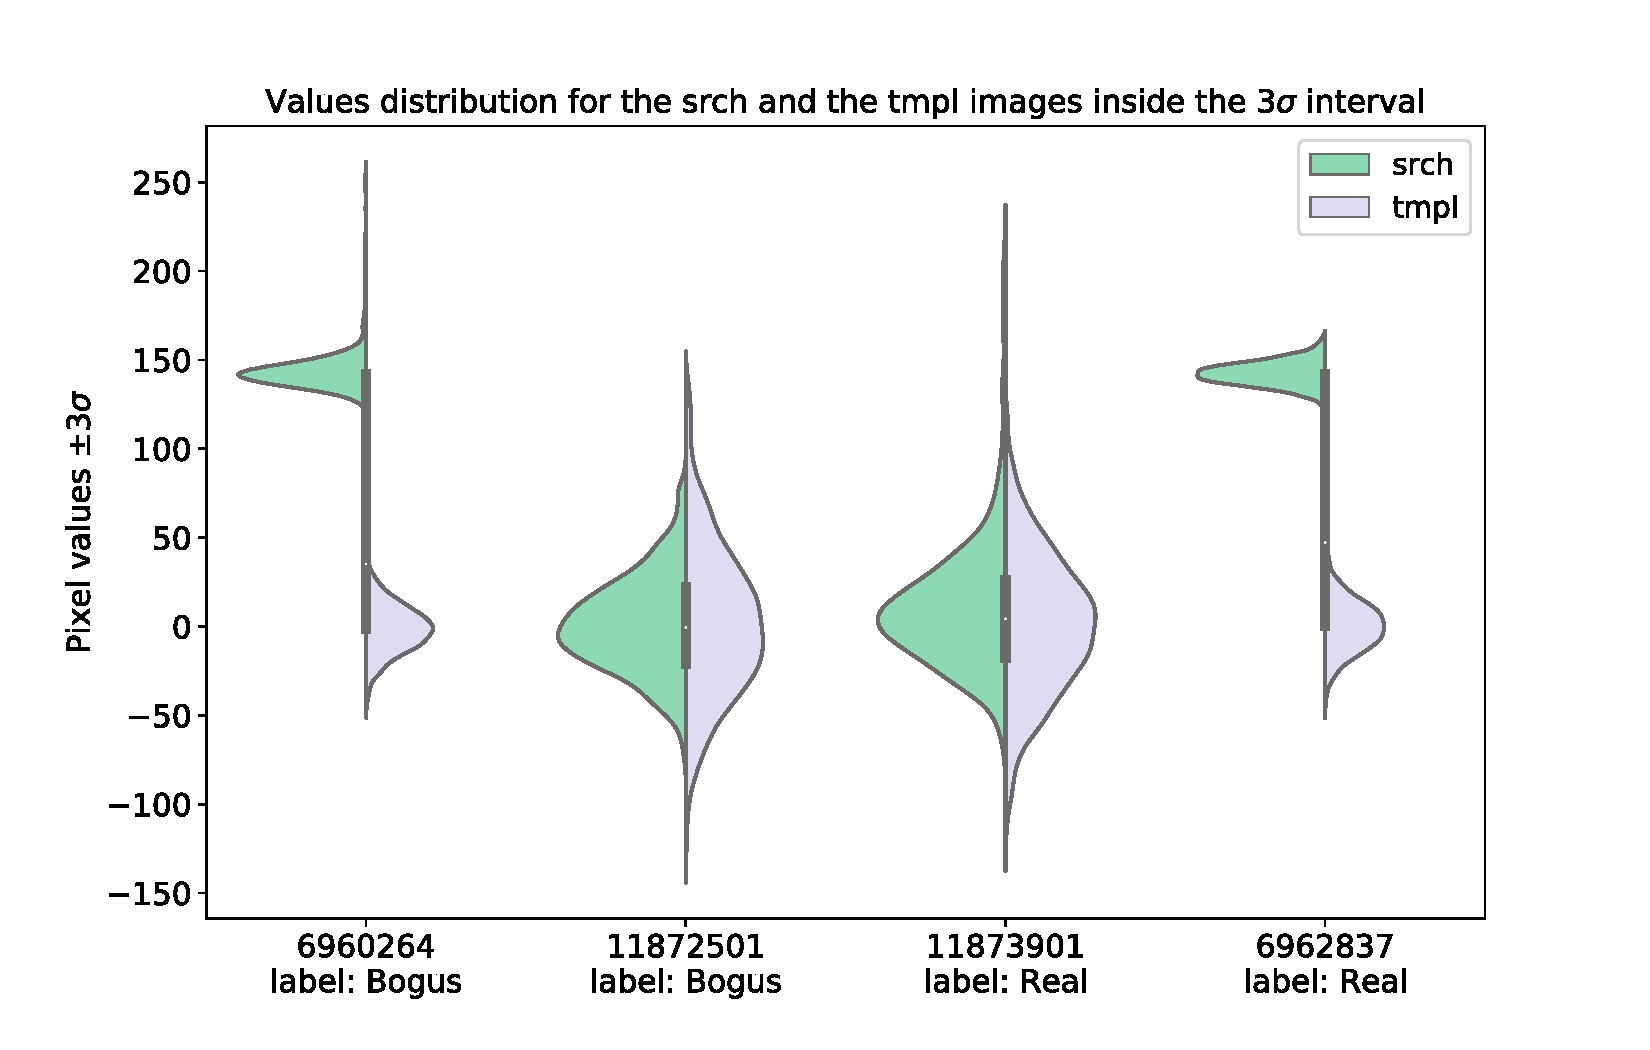
\includegraphics[width=0.6\linewidth]{
    figures/violin_plot.pdf}
    \caption{Violin plot of pixel values inside the $\mu \pm 3\sigma$ interval for \textit{srch} and \textit{temp} image of %Quantitative representation of 
    the data shown in \autoref{fig:examples_no_normalization} (before normalization). These values were scaled between $0$ and $1$. Left and right curve correspond to \textit{srch} and \textit{temp} distribution of values respectively. The distribution of values correspond to the same shown in \autoref{fig:histobeforenormalizarion} for \textit{srch} and \textit{temp}, the green and purple colors has its correspondence to \autoref{fig:histobeforenormalizarion}.}
    \label{fig:violinplot}
\end{figure*}



\begin{figure*}[h]
    \centering
    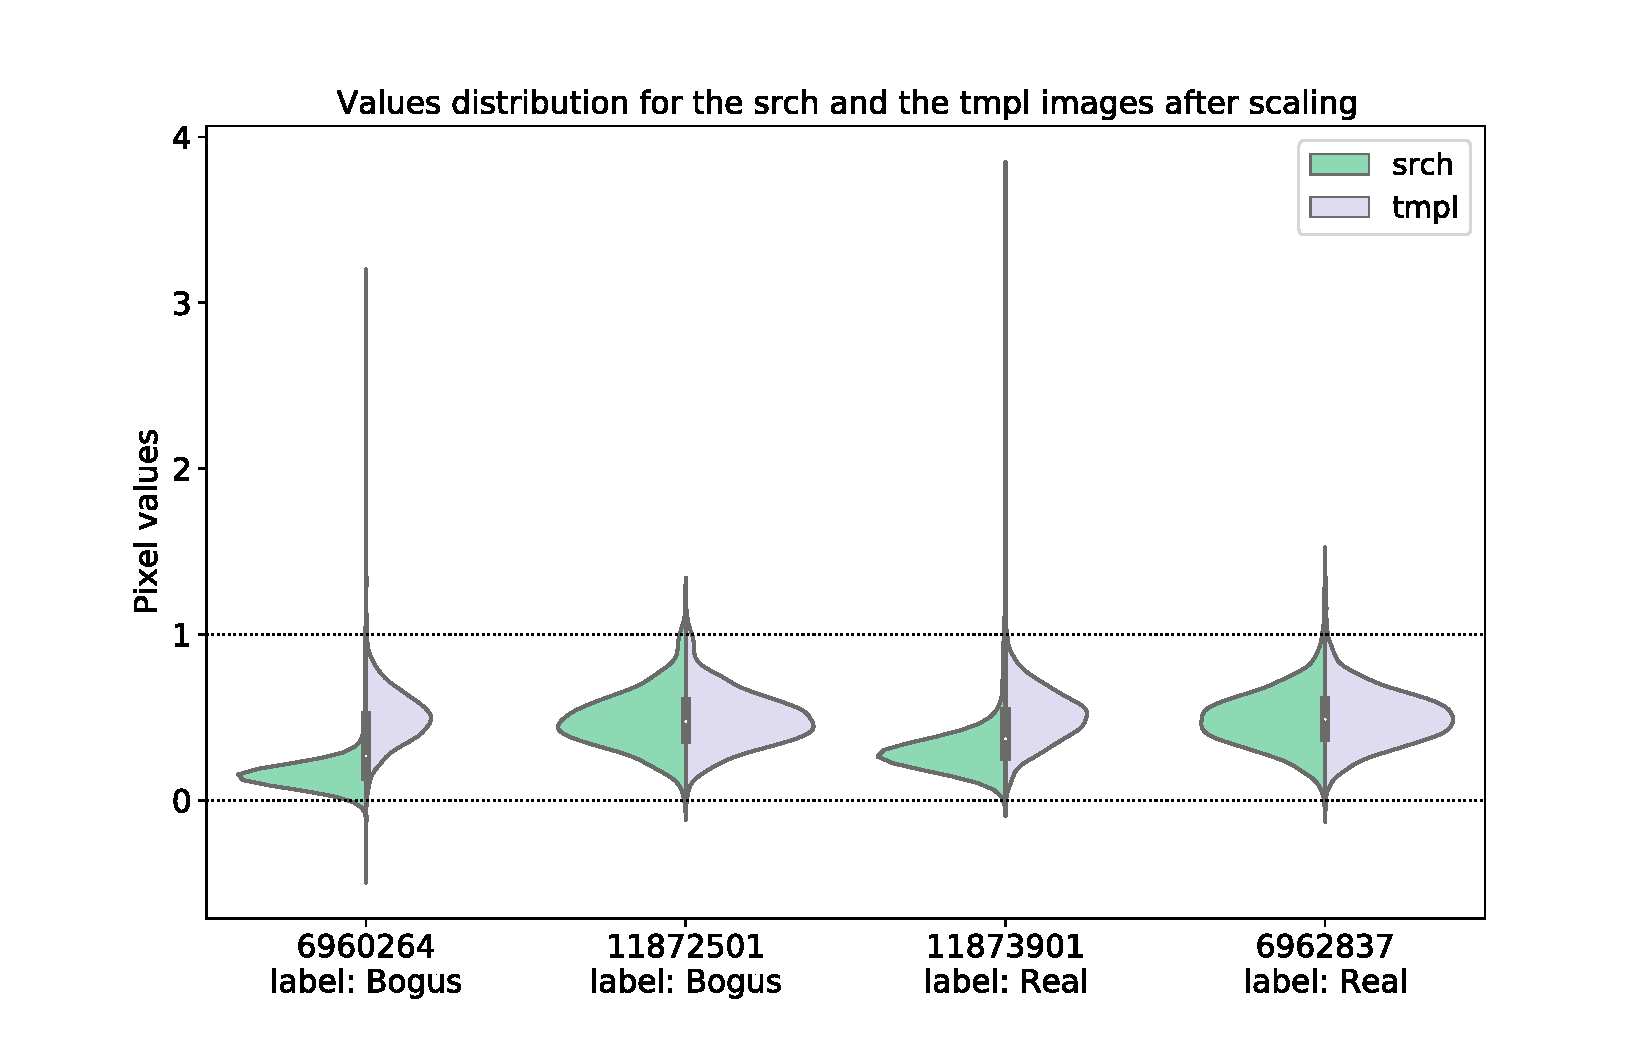
\includegraphics[width=0.6\linewidth]{
    figures/violin_plot_scaling.pdf}
    \caption{Violin plot of pixel values for \textit{srch} and \textit{temp} image of %Quantitative representation of 
    the data shown in \autoref{fig:examples_no_normalization} (after normalization). Values between the vertical lines in $0$ and $1$ were mapped to the values in \autoref{fig:violinplot}. Negative values and above $1$ correspond to the scaled values outside the $3\sigma$ clip. }
    \label{fig:violinplotscaling}
\end{figure*}

\clearpage


% \begin{itemize}
% \item \mintinline{c}/Conv2D/:
% % \subsubsection{\mintinline{c}/Conv2D/}
% According to the documentation of Convolutional layers in \url{https://keras.io/api/layers/convolution\_layers/convolution2d/}. The first parameter (\mintinline{c}/filter = 1 or 16 or 32 /) refers to the number of filters that the layer is going to learn. The outer layers learn less from the data than the inner layers. The second parameter (\mintinline{c}/kernel_size = [5,5]/) refers to the width and height of the filter that is multiplying the input data, the elements of the filter are the weights. The third parameter (\mintinline{c}/padding = "valid"/) define the way that the filter is going to sweep the input data, \mintinline{c}/"valid"/ refers that the operation between filter and input data is possible only if all the elements of the filters have a corresponding element in the input data. With this parameter the size of the output data is going to be smaller than the input. The latter parameters used here is the \mintinline{c}/activation = "relu"/,``Rectified Linear Unit''. The output data, know as feature map, is pass through the activation function to get the output layer.
% %to get the bias. 
% % The \mintinline{c}/"relu"/ function is defined as:
% % \begin{equation*}
% % ReLU = 
% % \begin{cases}
% %     0, & x\le0\\
% %     x, & x>0
% % \end{cases}
% % \end{equation*}
% %The ReLU is an efficient activation function that improves the performance of the Neural Network. [\cite{DBLP:journals/corr/abs-1803-08375, 10.5555/2999134.2999257, Dieleman_2015}]

% %\item \mintinline{c}/Conv2D/:
% %Reduces the size of the output given in \mintinline{c}/Conv2D/ by a given matrix size, selecting the maximum value of the window where the pool matrix fit within the matrix output of the \mintinline{c}/Conv2D/. The size reduction is done by applying an aggregation function to the output of the previous layer, in this case to choose the maximum value within a specific windows across all the output, small translation could lead to the same maximum values. This layer add an approximately invariance on small translations. \citep{Gieseke_2017}

% \item \mintinline{c}/Dropout/:
% Eliminates randomly output values of the previous layer, the CNN model would not learn features that are not relevant to unseen data. In this way a better performance on the training data, compared to the validation or testing data would be avoided, the called \textit{overfitting}. The model would be able to predicted successfully with the same or similar rate in both data sets. [\cite{Dieleman_2015, Gieseke_2017}]

% \item \mintinline{c}/Flatten/:
% Reduces the dimensions of the data to be a one dimension array.

% \item \mintinline{c}/Dense/:
% Make the previous layer all fully connected with the next layer.

% \end{itemize}
